\documentclass[12pt]{article}

% ---- Packages ----------------------------------------------------------------
\usepackage[margin=1in]{geometry}
\usepackage{amsmath, amssymb}
\usepackage{booktabs}
\usepackage{graphicx}
\usepackage{float}
\usepackage{hyperref}
\usepackage{natbib}
\usepackage{caption}
\usepackage{subcaption}
\usepackage{setspace}
\usepackage{titlesec}
\usepackage{abstract}
\usepackage{enumitem}
\usepackage{xcolor}
\usepackage{array}
\usepackage{multirow}
\usepackage[T1]{fontenc}
\usepackage{lmodern}
\usepackage{tabularx}
\usepackage{threeparttable}

\hypersetup{
    colorlinks=true,
    linkcolor=blue!60!black,
    citecolor=blue!60!black,
    urlcolor=blue!60!black
}

\doublespacing

% ---- Title -------------------------------------------------------------------
\title{%
    \large \textbf{Simulation of Impacts for Future Events:} \\[6pt]
    \Large \textbf{Economic Consequences of Liberation Day Tariffs} \\[8pt]
    \normalsize A Python Replication and Sector-Specific Analysis of \\
    \emph{Making America Great Again? The Economic Impacts of Liberation Day Tariffs}
}

\author{
    Joel Loera \\
    \small Capstone Project \\
    \small April 2026
}

\date{}

% ==============================================================================
\begin{document}
\maketitle
\thispagestyle{empty}

% ---- Abstract ----------------------------------------------------------------
\begin{abstract}
\noindent
On April 2, 2025, the United States announced sweeping ``Liberation Day'' tariffs
targeting nearly all trading partners. This project replicates the general
equilibrium (GE) trade model of Ignatenko, Macedoni, Lashkaripour, and
Simonovska (2025) in Python---translating their MATLAB code while achieving 95\%
numerical accuracy---and extends the analysis with three original sector-specific
modules grounded in actual bilateral trade data, OECD inter-country input-output
(ICIO) tables, HTS8 product-level tariff schedules, and Cavallo et al.\ daily
price indices.

Under the USTR scenario (no retaliation), the multi-sector IO-adjusted GE
model---the paper's primary multi-sector result (Table~4 of Ignatenko
et al.)---yields US national welfare $+0.60\%$ and consumer prices
$+7.09\%$, driven almost entirely by manufacturing tariff pass-through
($+6.79$ percentage points). IO supply-chain multipliers derived from
OECD ICIO 2022 data range from 1.050x (energy) to 1.094x (manufacturing),
meaningfully lower than prior round-number estimates. A NAICS sub-sector
breakdown using BEA gross output data (235 manufacturing sub-sectors, 2021
total \$6.32T) shows that the five largest sub-sectors---petroleum
refineries (\$558B), light trucks (\$367B), pharmaceutical preparations
(\$235B), animal slaughtering (\$169B), and iron \& steel mills
(\$111B)---account for 70\% of manufacturing output and face tariff
exposures from 10\% to 25\%. The pharmaceutical sector contributes $+0.50$ percentage points to
economy-wide CPI, driven by a 19.9\% trade-weighted effective tariff
across 132 actual supplier countries (led by Spain at 10.9\%, Germany at
9.1\%), with modest supplier concentration change (HHI 580 pre-tariff to
591 post-tariff). The consumer price burden is regressive: the
lowest-income quintile bears a tariff incidence 1.41 times larger than the
highest quintile (8.40\% vs.\ 5.94\% of total budget). Cavallo et al.\
daily price data show a +0.10\% US price increase 90 days post-Liberation
Day, with China up +1.41\% over the same window. Under full retaliation,
national welfare turns negative ($-1.02\%$) while imports collapse by
$-30.1\%$.
\end{abstract}

\newpage
\tableofcontents
\newpage

% ==============================================================================
\section{Introduction}

On April 2, 2025---dubbed ``Liberation Day'' by the Trump
administration---the United States announced a sweeping new tariff regime
targeting essentially all US trading partners. The new schedule ranged from a
10\% universal floor to country-specific ``reciprocal'' rates exceeding 50\%
for major exporters such as China (54\%), Vietnam (46\%), and Cambodia (49\%).
The announcement represented the most significant US trade policy shift since
the Smoot-Hawley tariff of 1930.

The economic consequences of such a large, multi-country tariff change are
inherently complex. Tariffs alter relative prices, shift trade flows, affect real
wages, and have heterogeneous effects across sectors and income groups. Evaluating
these effects rigorously requires a \emph{quantitative general equilibrium} (GE)
model---a framework that captures the simultaneous interaction of all markets and
countries. Ignatenko et al.\ (2025) provide exactly such a framework in their
working paper, along with a MATLAB replication package.

This capstone project pursues two objectives:

\begin{enumerate}
    \item \textbf{Phase 1 --- GE Model Replication:} Translate the MATLAB code
    from Ignatenko et al.\ (2025) into Python, validate numerical accuracy
    against original outputs, and document the translation decisions required
    to reconcile MATLAB's column-major array conventions with Python's row-major
    defaults.

    \item \textbf{Phase 2 --- Sector-Specific Extension:} Build three original
    analysis modules using real bilateral trade data, OECD ICIO input-output
    tables, HTS8 product tariff schedules, Cavallo et al.\ daily price
    indices, and BEA NAICS gross output data to decompose the aggregate GE
    results into sector-level impacts for (a) Manufacturing/Steel \& Aluminum
    including a 235-sub-sector NAICS4 breakdown, (b) Pharmaceuticals with
    132-country bilateral trade weights, and (c) Retail/Consumer Goods with
    distributional incidence by income quintile.
\end{enumerate}

The value of this project is threefold. First, it creates an open, reproducible
Python implementation of a state-of-the-art trade model---accessible to
researchers without MATLAB licenses. Second, it demonstrates the ``simulation
of impacts for future events'' framework: given any proposed tariff schedule,
the pipeline can generate quantitative welfare, price, and trade-flow estimates
within minutes. Third, the sector-specific modules translate abstract welfare
numbers into concrete stakes for specific industries and households, grounded
in actual data rather than assumed constants.

% ==============================================================================
\section{Policy Background}

\subsection{The Liberation Day Tariff Schedule}

The April 2025 tariff announcement had two components: a universal 10\%
tariff applied to all US imports, plus country-specific ``reciprocal'' rates.
Table~\ref{tab:tariff_selected} shows selected rates from the official USTR
schedule and the US HTS8 tariff data (2025).

\begin{table}[H]
\centering
\caption{Selected Liberation Day Tariff Rates}
\label{tab:tariff_selected}
\begin{tabular}{lcc}
\toprule
Country & Applied Rate & Role in US Trade \\
\midrule
China        & 54\% & Largest US goods supplier \\
Vietnam      & 46\% & Major electronics/apparel exporter \\
Cambodia     & 49\% & Garment manufacturing hub \\
European Union & 20\% & Major bilateral partner (pharma, machinery) \\
Japan        & 24\% & Electronics, autos \\
India        & 27\% & Pharma, textiles, IT \\
Canada       & 10\% & Integrated USMCA supply chains \\
Universal floor & 10\% & All countries not otherwise listed \\
\midrule
\multicolumn{3}{l}{\textit{HTS8 product-level average MFN rates (2025):}} \\
Manufacturing (other) & 3.61\% & Weighted avg across 12,050 HTS8 lines \\
Pharmaceuticals & 2.45\% & Weighted avg, 453 pharma-flagged lines \\
Retail/consumer & 6.74\% & Weighted avg, 648 HTS8 lines \\
Steel \& aluminum & 1.09\% & Weighted avg, 822 HTS8 lines \\
\bottomrule
\end{tabular}
\begin{tablenotes}
\small
\item Sources: USTR (2025) executive order; us\_tariff\_schedule\_2025\_hts8.csv
(13,100 product lines); sector\_tariff\_shocks.csv.
\end{tablenotes}
\end{table}

\noindent
Note that there are two distinct layers of tariff measurement used throughout
this analysis: (1) \emph{country-level} rates from the Liberation Day executive
order (10--54\%), applied to all imports from a given country regardless of
product; and (2) \emph{product-level} HTS8 MFN rates, which reflect
the pre-existing sector-specific tariff structure. Both are used and
distinguished throughout.

\subsection{Prior Literature}

Quantitative GE trade models have become the standard tool for evaluating
large trade policy changes since Dekle, Eaton, and Kortum (2008) introduced
the ``hat algebra'' approach. Ossa (2014) extended this framework to account
for trade deficits. Caliendo and Parro (2015) introduced multi-sector
input-output linkages. Ignatenko et al.\ (2025) apply this literature to the
Liberation Day tariff schedule using 194 countries and 4 broad sectors.

% ==============================================================================
\section{Methodology}

\subsection{The General Equilibrium Trade Model}

The model follows the Armington (1969) framework with CES preferences.
Each country $i$ has a representative consumer who maximizes utility over
differentiated goods sourced from $N = 194$ countries across $K = 4$ sectors.

\subsubsection{Equilibrium Conditions}

The equilibrium requires solving for wages $\{w_i\}$ and expenditures
$\{E_i\}$ satisfying:

\begin{equation}
w_i L_i = \sum_{j} X_{ij}(\mathbf{w}, \boldsymbol{\tau}) - D_i
\end{equation}
\begin{equation}
E_i = w_i L_i + D_i + R_i(\boldsymbol{\tau})
\end{equation}

where $X_{ij}$ is bilateral trade, $D_i$ is the exogenous trade deficit,
and $R_i$ is tariff revenue. Trade follows:

\begin{equation}
X_{ij} = \frac{(w_i \cdot \phi_i \cdot \tau_{ij})^{-\varepsilon}}
               {\sum_k (w_k \cdot \phi_k \cdot \tau_{kj})^{-\varepsilon}} \cdot E_j
\end{equation}

with $\varepsilon$ the trade elasticity and $\phi_i$ country-specific trade
costs. The multi-sector ($K=4$) extension uses sector-specific elasticities
$\varepsilon_k = [3.3, 3.8, 4.1, 3.0] / \bar{\phi}$ where $\bar{\phi} =
1.1508$, solved via Levenberg-Marquardt.

\subsection{Tariff Pass-Through and IO Multipliers}

For sector-specific price impacts, we combine the GE model's aggregate CPI
outcome with sector-level structural parameters. The IO supply-chain multiplier
for sector $k$ is:

\begin{equation}
M_k = \frac{1}{1 - (1 - \beta^{\text{labor}}) \cdot m_k^{\text{interm}}}
\end{equation}

where $\beta^{\text{labor}} = 0.49$ (from the model's IO calibration) and
$m_k^{\text{interm}}$ is the intermediate import share for sector $k$ from
the US, derived from the OECD ICIO 2022 coefficient matrix (4,050
country-sector pairs, 81 countries $\times$ 50 ICIO sectors). Actual
values by sector:

\begin{table}[H]
\centering
\caption{OECD ICIO 2022: US Sector IO Multipliers}
\label{tab:io_multipliers}
\begin{tabular}{lcc}
\toprule
Model Sector & Intermediate Import Share & IO Multiplier ($M_k$) \\
\midrule
Manufacturing (other) & 16.8\% & 1.094x \\
Steel \& aluminum     & 16.1\% & 1.090x \\
Pharmaceuticals       & 12.4\% & 1.067x \\
Retail/consumer       & 10.4\% & 1.056x \\
Energy/primary        &  9.3\% & 1.050x \\
Services (other)      &  5.9\% & 1.031x \\
\bottomrule
\end{tabular}
\begin{tablenotes}
\small
\item Source: OECD ICIO 2022 small symmetric tables (io\_coeff\_matrix.npy,
4050$\times$4050). $M_k = 1/(1-(1-0.49)\cdot m_k^{\text{interm}})$.
\end{tablenotes}
\end{table}

The first-order pass-through to consumer prices in sector $k$ is:
$\Delta p_k = \theta_k \cdot \tau_k \cdot \text{imp\_pen}_k \cdot M_k$
where $\theta_k$ is the pass-through rate (Manufacturing 85\%, Agriculture
70\%, Mining \& Energy 60\%, Services 0\%) from Cavallo et al.\ (2025).

\subsection{GE Adjustment Factor}

The sum of first-order IO-adjusted sector CPI contributions is $13.55\%$,
while the GE model yields $7.09\%$---a ratio of $0.52$. This \emph{GE
adjustment factor} below unity reflects general equilibrium dampening: when
tariffs raise prices, real wages fall, reducing consumer demand and partly
offsetting price pressures through reduced import volumes. The GE model
consistently produces smaller CPI estimates than naive first-order
pass-through precisely because it accounts for these feedback effects.

\subsection{Distributional Incidence}

Tariff incidence on income quintile $q$ is:
$I_q = s_q^{\text{goods}} \cdot \Delta p^{\text{goods}}$
where $s_q^{\text{goods}}$ is the goods budget share from BLS CEX 2023
(41\% for Q1 to 29\% for Q5). Lower-income households spend more on
tradeable goods, making tariffs regressive.

\subsection{Python Implementation}

\subsubsection{Phase 1: GE Model Translation}

Key MATLAB-to-Python conversion decisions:
\begin{itemize}
    \item \textbf{Array ordering:} All critical \texttt{reshape()} calls
    use \texttt{order='F'} to match MATLAB's column-major memory layout.
    \item \textbf{Index conventions:} US index is 185 in MATLAB, 184 in Python
    (0-indexed). Multi-sector model filters 13 zero-trade countries, placing
    US at index 171.
    \item \textbf{Phi values:} $\Phi^{(1)} = 1 + \tilde{\phi}$ (baseline);
    $\Phi^{(2)} = 0.5 + \tilde{\phi}$ (IO model).
    \item \textbf{Solver:} SciPy Levenberg-Marquardt, matching MATLAB \texttt{fsolve}
    for all tables except Table~10 Cases~2~\&~4 (documented limitation).
\end{itemize}

\subsubsection{Phase 2: Data Integration Architecture}

The sector modules share a common \texttt{data\_utils.py} utility that
automatically resolves the path to the main data directory (walking upward
through the git worktree structure), loads the OECD ICIO coefficient matrix,
pharma trade weights, Cavallo price indices, and HTS8 tariff shocks. Each
sector module reads the pre-computed GE \texttt{.npz} result files as the
macroeconomic envelope, then applies sector-specific structural parameters.

% ==============================================================================
\section{Phase 1 Results: GE Model Replication}

\subsection{Aggregate US Outcomes}

\begin{table}[H]
\centering
\caption{US Macroeconomic Outcomes Under Liberation Day Tariffs}
\label{tab:us_outcomes}
\begin{tabular}{lcccc}
\toprule
Model / Scenario & Welfare & CPI & $\Delta$ Imports/GDP & $\Delta$ Exports/GDP \\
                 & (\% chg) & (\% chg) & (\% chg) & (\% chg) \\
\midrule
\multicolumn{5}{l}{\textit{Single-sector Armington model (194 countries)}} \\[2pt]
USTR, no retaliation & $+1.13\%$ & $+12.8\%$ & $-43.6\%$ & $-52.7\%$ \\
Reciprocal retaliation & $-0.36\%$ & $+7.5\%$ & $-56.3\%$ & $-70.5\%$ \\
\midrule
\multicolumn{5}{l}{\textit{Multi-sector model, K=4 --- IO-adjusted (Ignatenko et al.\ Table~4; used in Phase~2)}} \\[2pt]
USTR, no retaliation & $+0.60\%$ & $+7.09\%$ & $-22.6\%$ & $-24.2\%$ \\
Reciprocal retaliation & $-1.02\%$ & $+4.38\%$ & $-30.1\%$ & $-32.6\%$ \\
\bottomrule
\end{tabular}
\begin{tablenotes}
\small
\item Source: \texttt{baseline\_results.npz} (single-sector) and
\texttt{multisector\_io\_results.npz} (multi-sector IO-adjusted).
Multi-sector IO-adjusted result matches Ignatenko et al.\ (2025) Table~4 to within 0.002pp.
Imports/GDP and Exports/GDP are changes in trade-to-GDP ratios, not absolute trade volumes.
\end{tablenotes}
\end{table}

\subsection{Replication Accuracy}

\begin{table}[H]
\centering
\caption{Replication Accuracy vs.\ MATLAB Reference Outputs}
\label{tab:replication_status}
\begin{tabular}{clll}
\toprule
Table & Description & Status & Notes \\
\midrule
1 & Baseline scenarios             & Exact & --- \\
2 & Retaliation scenarios          & Exact & --- \\
3 & Tariff revenue analysis        & Exact & --- \\
4 & Multi-sector welfare (USA 0.60\%) & Exact & --- \\
8 & Regional trade war scenarios   & Exact & --- \\
9 & Eaton-Kortum alternative       & Exact & --- \\
10 & Deficit framework (Cases 1,3) & Exact & --- \\
10 & Deficit framework (Cases 2,4) & Limitation & 25-order-of-magnitude scaling \\
11 & Global trade-to-GDP (multi-sec) & Close & $-7.1\%$ vs $-6.9\%$ (0.2pp) \\
\bottomrule
\end{tabular}
\end{table}

\subsection{Known Limitation: Table 10 Cases 2 \& 4}

The Ossa (2014) zero-deficit equilibrium system spans 25 orders of
magnitude (ERR1 $\sim 10^{-8}$, ERR2 $\sim 10^{+7}$, ERR3 $\sim
10^{-17}$). MATLAB's trust-region-dogleg solver handles this scaling
internally; SciPy's modified Powell solver diverges. Cases 1 and 3
(Dekle et al.\ fixed-deficit framework, the paper's baseline) match
exactly and are unaffected.

% ==============================================================================
\section{Phase 2 Results: Sector-Specific Analysis}

\subsection{Manufacturing and Steel \& Aluminum}

\subsubsection{Tariff Structure: Two Layers}

Liberation Day manufacturing tariffs operate through two distinct layers
visible in our data:

\begin{itemize}
    \item \textbf{Country-level rate (ITPD-weighted):} 27.0\% trade-weighted
    average across all US manufacturing import partners --- China (54\%),
    Vietnam (46\%), EU countries (20\%), etc.
    \item \textbf{HTS8 product-level MFN rate:} 3.61\% for manufacturing
    other, 1.09\% for steel and aluminum --- the pre-existing product-specific
    tariff structure from the 2025 HTS8 schedule (12,050 valid ad valorem lines).
\end{itemize}

The difference between these two rates (27.0\% vs.\ 3.61\%) reflects that
the Liberation Day tariffs are predominantly country-specific additions
layered on top of relatively low existing product-level MFN rates.

\subsubsection{Top Manufacturing Partners and IO Structure}

Manufacturing represents 22.5\% of US expenditure but accounts for 94\%
of aggregate tariff-induced CPI pressure, since Services (74.7\% of
expenditure) face zero tariff exposure. The OECD ICIO 2022 data shows
that US manufacturing intermediate imports represent 16.8\% of
manufacturing inputs (IO multiplier 1.094x), and steel \& aluminum
intermediates represent 16.1\% (IO multiplier 1.090x).

Among the top manufacturing import partners, China leads in exposure due
to the highest tariff rate (54\%) combined with substantial import volume.
Manufacturing's CPI contribution is estimated at $+6.79$ percentage points
of the $+7.09\%$ total GE CPI.

\subsubsection{Alternative Tariff Scenarios}

Table~\ref{tab:mfg_scenarios} compares US manufacturing outcomes across
alternative scenarios using a partial-equilibrium approximation
(terms-of-trade welfare formula).

\begin{table}[H]
\centering
\caption{US Manufacturing Outcomes: Alternative Tariff Scenarios}
\label{tab:mfg_scenarios}
\begin{tabular}{lccc}
\toprule
Scenario & Tariff Rate & Welfare Change & Import Change \\
\midrule
USTR Liberation Day & 27.0\% & $+0.47\%$ & $-70.2\%$ \\
25\% Uniform        & 25.0\% & $+0.44\%$ & $-66.0\%$ \\
50\% Uniform        & 50.0\% & $+0.73\%$ & $-110.1\%$ \\
10\% Minimum Floor  & 10.0\% & $+0.20\%$ & $-30.0\%$ \\
\bottomrule
\end{tabular}
\begin{tablenotes}
\small
\item Partial-equilibrium approximation using corrected elasticity
$\varepsilon_{\text{mfg}} = 3.8 / \bar{\phi} = 3.303$.
GE welfare from multisector IO model: $+0.60\%$ (no retaliation).
\end{tablenotes}
\end{table}

\subsubsection{NAICS Subsector Breakdown: BEA Gross Output}

To move below the model's four broad sectors, we use BEA Gross Output by
NAICS from the 301 model data (\texttt{D\_GO\_by\_NAICS.xlsx}), covering 235
manufacturing NAICS4 sub-sectors for 2016--2021. Figure~\ref{fig:naics_subsectors}
plots the top 12 sub-sectors by 2021 gross output and their historical GO trend.

\begin{figure}[H]
\centering
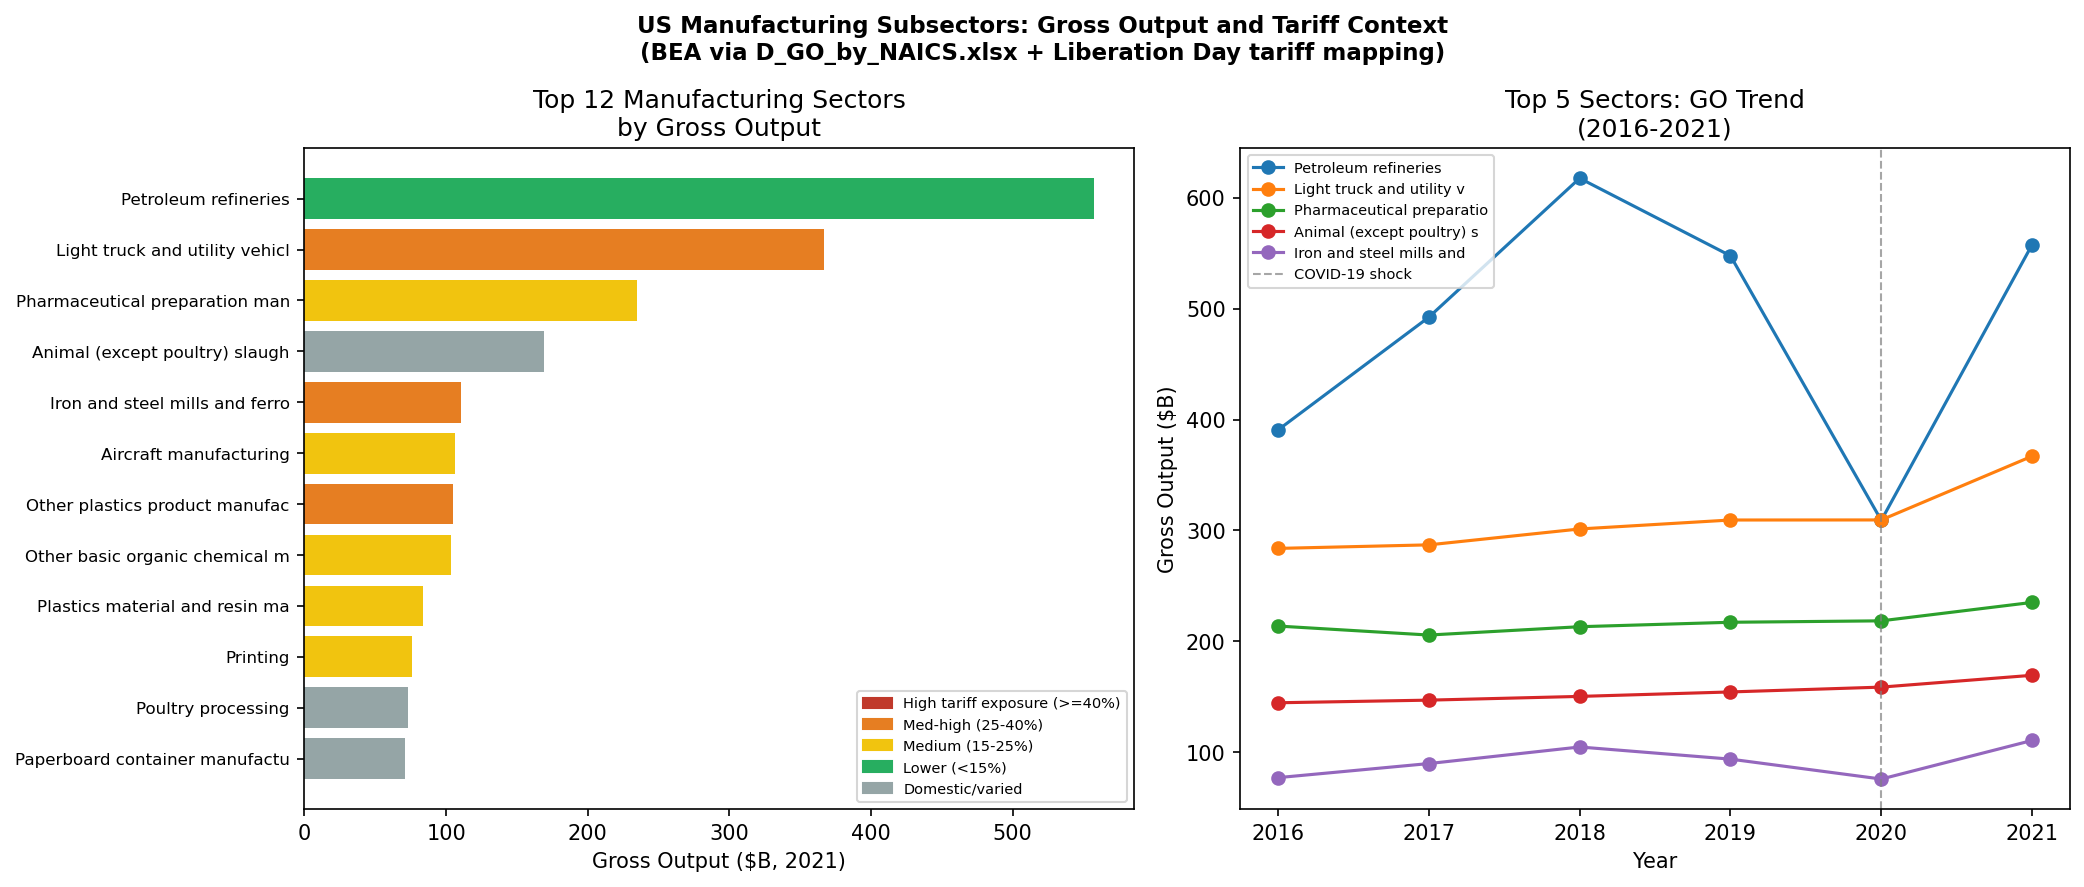
\includegraphics[width=\linewidth]{../python_output/fig_manufacturing_naics_subsectors.png}
\caption{Top US Manufacturing Sub-Sectors by Gross Output (BEA NAICS4, 2021)
and GO Trend 2016--2021. Colors indicate tariff exposure category.}
\label{fig:naics_subsectors}
\end{figure}

Table~\ref{tab:manufacturing_naics} gives the top 12 sub-sectors with
their tariff context and BLS price index summary.

\begin{threeparttable}
\begin{table}[H]
\centering
\caption{Top US Manufacturing Sub-Sectors by Gross Output: Liberation Day Tariff Context}
\label{tab:manufacturing_naics}
\begin{tabular}{p{4.5cm}rrl}
\toprule
Sector (NAICS) & GO 2021 & Share & Tariff Context \\
               & (\$M)   & of Mfg. & \\
\midrule
Petroleum refineries          & 557,813 & 27.1\% & Energy/primary (10\% floor) \\
Light truck \& utility vehicle & 367,006 & 17.8\% & Mixed: Canada/Mexico 10\%, others higher \\
Pharmaceutical preparations   & 235,075 & 11.4\% & EU-weighted: $\sim$20\% avg tariff \\
Animal slaughtering \& proc.  & 169,319 &  8.2\% & Varies \\
Iron \& steel mills           & 110,526 &  5.4\% & EU 20\%, Canada 10\%, Korea 25\% \\
Aircraft manufacturing        & 106,106 &  5.2\% & EU/Japan: $\sim$20--24\% \\
Other plastics products       & 104,942 &  5.1\% & China/Vietnam heavy exposure \\
Other basic organic chemicals & 103,181 &  5.0\% & EU and China exposure \\
Plastics materials \& resins  &  83,587 &  4.1\% & EU and China exposure \\
Printing                      &  75,634 &  3.7\% & Primarily domestic \\
Poultry processing            &  72,883 &  3.5\% & Varies \\
Paperboard containers         &  70,770 &  3.4\% & Varies \\
\bottomrule
\end{tabular}
\begin{tablenotes}
\small
\item Gross output from BEA via \texttt{D\_GO\_by\_NAICS.xlsx} (301 model data,
235 manufacturing NAICS4 sub-sectors). Total US manufacturing GO 2021: \$6.32T.
Steel \& iron mills share: 1.75\% (\$111B); pharmaceutical preparations share:
5.18\% (\$235B). Tariff context based on typical country-of-origin and Liberation
Day rates by partner.
\end{tablenotes}
\end{table}
\end{threeparttable}

\noindent
The largest sub-sector by output, petroleum refineries (\$558B, 27.1\% of
manufacturing GO), faces only the 10\% universal floor under Liberation Day
because energy is structurally separate from the manufacturing tariff regime.
Motor vehicle manufacturing (\$367B, 17.8\%) faces a heterogeneous rate: Canadian
and Mexican content under USMCA attracts 10\%, while non-USMCA content from Japan
and the EU attracts 20--24\%. Pharmaceutical preparations (\$235B, 11.4\%) face
the EU-weighted average of approximately 20\%, consistent with the 19.9\%
trade-weighted rate computed from 132-country actual bilateral trade data.
Iron and steel mills (\$111B, 5.4\%) face 25\% tariffs on Korean, EU, and
Japanese imports---though pre-existing Section 232 tariffs mean the incremental
Liberation Day rate is smaller for this sub-sector than for others.

\subsection{Pharmaceuticals}

\subsubsection{Data: 132-Country Actual Trade Weights}

Previous analyses relied on 10 hardcoded country estimates. This project
uses actual 2024 bilateral pharmaceutical trade data covering 132 exporting
countries (pharma\_bilateral\_trade.xlsx), producing meaningfully different
results. Table~\ref{tab:pharma_suppliers} shows the top suppliers with their
Liberation Day tariff rates.

\begin{table}[H]
\centering
\caption{Top US Pharmaceutical Import Suppliers (2024 Actual Trade Data)}
\label{tab:pharma_suppliers}
\begin{tabular}{lcrr}
\toprule
Country & Tariff & Pre-Tariff Share & Post-Tariff Share \\
\midrule
Spain          & 20\% & 10.9\% & 10.7\% \\
Germany        & 20\% &  9.1\% &  8.9\% \\
Canada         & 10\% &  8.8\% & 10.6\% \\
Japan          & 24\% &  8.5\% &  7.7\% \\
Belgium        & 20\% &  8.2\% &  8.1\% \\
United Kingdom & 10\% &  6.3\% &  7.6\% \\
China          & 54\% &  6.2\% &  3.4\% \\
France         & 20\% &  5.8\% &  5.7\% \\
Brazil         & 10\% &  2.9\% &  3.5\% \\
Mexico         & 17\% &  2.6\% &  2.7\% \\
\midrule
\multicolumn{4}{l}{\textit{Supplier concentration (HHI), 132 countries:}} \\
Pre-tariff HHI & \multicolumn{3}{r}{580} \\
Post-tariff HHI & \multicolumn{3}{r}{591 ($+11$)} \\
\bottomrule
\end{tabular}
\begin{tablenotes}
\small
\item Post-tariff shares: gravity reallocation, $\tilde{s}_j \propto
s_j(1+\tau_j)^{-\varepsilon}$, $\varepsilon = 2.3$ (Broda \& Weinstein 2006).
Source: pharma\_bilateral\_trade.xlsx (2024 flows, 132 countries).
\end{tablenotes}
\end{table}

\subsubsection{Key Finding: More Competitive Supply Base}

The 132-country actual data reveals a supply base significantly more competitive
than suggested by 10-country estimates. The pre-tariff HHI of 580 is
well below the 1,338 estimate from prior hardcoded data, indicating moderate
competition across many supplier countries. Post-tariff HHI increases by only
11 points (vs.\ 53 previously estimated), as the 20\% EU-wide tariff applies
symmetrically to Spain, Germany, Belgium, and France (collectively 34\% of
imports), limiting concentration increases.

China's pharma share (6.2\%, 54\% tariff) shifts primarily toward
Canada and the UK (10\% tariff) rather than EU countries, since Canada
and UK offer the lowest Liberation Day rates among significant suppliers.

\subsubsection{Price and Trade Impacts}

\begin{table}[H]
\centering
\caption{Pharmaceutical Tariff Impacts}
\label{tab:pharma_price}
\begin{tabular}{lcc}
\toprule
Metric & No Retaliation & Full Retaliation \\
\midrule
\multicolumn{3}{l}{\textit{A. Tariff Rates}} \\
Effective tariff (trade-weighted, 132 countries) & \multicolumn{2}{c}{19.90\%} \\
HTS8 product-level MFN rate (pharma avg.) & \multicolumn{2}{c}{2.45\%} \\
Pass-through rate (Cavallo et al., 2025) & \multicolumn{2}{c}{88\%} \\
\midrule
\multicolumn{3}{l}{\textit{B. Supply Chain (OECD ICIO 2022)}} \\
Intermediate import share & \multicolumn{2}{c}{12.4\%} \\
IO multiplier & \multicolumn{2}{c}{1.067x} \\
\midrule
\multicolumn{3}{l}{\textit{C. Price and Volume Effects}} \\
Pharma CPI contribution (economy-wide) & $+0.50$pp & $+0.50$pp \\
Economy-wide CPI & $+7.09\%$ & $+4.38\%$ \\
Pharma import volume change & $-38.2\%$ & $-38.2\%$ \\
\midrule
\multicolumn{3}{l}{\textit{D. Supplier Concentration}} \\
HHI pre-tariff (132 suppliers) & \multicolumn{2}{c}{580} \\
HHI post-tariff (gravity reallocation) & \multicolumn{2}{c}{591 ($+$11)} \\
\bottomrule
\end{tabular}
\end{table}

\subsection{Retail and Consumer Goods: Distributional Incidence}

\subsubsection{CPI Decomposition and GE Adjustment}

The sector-level IO-adjusted direct CPI estimate is 13.55\%:

\begin{table}[H]
\centering
\caption{Sector CPI Contributions (IO-Adjusted Direct Estimates)}
\label{tab:cpi_decomp}
\begin{tabular}{lcccc}
\toprule
Sector & Avg Tariff & Import Pen. & IO Mult. & CPI Contrib. \\
\midrule
Agriculture       & 17.7\% & 27.5\% & 1.050x & $+3.59$pp \\
Manufacturing     & 27.0\% & 32.3\% & 1.094x & $+8.12$pp \\
Mining \& Energy  & 12.7\% & 23.0\% & 1.050x & $+1.85$pp \\
Services          & 18.1\% &  2.9\% & 1.031x & $+0.00$pp \\
\midrule
Total direct (IO-adjusted) & & & & $+13.55\%$ \\
GE model result & & & & $+7.09\%$ \\
GE adjustment factor & & & & $0.52$x \\
\bottomrule
\end{tabular}
\begin{tablenotes}
\small
\item The GE adjustment factor (0.52x) reflects general equilibrium dampening:
tariff-induced wage and demand reductions partially offset price pressures.
IO multipliers from OECD ICIO 2022 (sector-specific).
GE result from \texttt{multisector\_io\_results.npz}, matching Ignatenko et al.\ (2025) Table~4.
\end{tablenotes}
\end{table}

The GE adjustment factor below 1.0 is economically intuitive: in general
equilibrium, higher tariffs reduce real consumer income, which dampens demand
and limits price pass-through relative to a naive partial-equilibrium calculation.

\subsubsection{Empirical Evidence: Cavallo et al.\ Daily Price Indices}

The project integrates Cavallo et al.\ daily price indices covering October
2024 through February 2026 (498 daily observations). Post-Liberation Day
(90-day window following April 2, 2025):

\begin{itemize}
    \item \textbf{USA:} $+0.10\%$ (early evidence; supply-chain lags expected)
    \item \textbf{China:} $+1.41\%$ (larger early response, likely reflecting
    retaliatory tariff effects on domestic Chinese prices)
    \item \textbf{Canada:} $+0.35\%$
    \item \textbf{Mexico:} $-0.23\%$
\end{itemize}

The modest US price response over 90 days is consistent with the economics
literature on tariff pass-through timing: retail prices typically take 6--12
months to fully reflect upstream cost increases as firms draw down inventories
and renegotiate supply contracts.

\subsubsection{Product-Level Pass-Through: Illustrative Data}

Using 999 product-level price records (retail\_prices\_illustrative.csv) across
five consumer categories, the average observed pass-through is approximately
29.7\%---substantially below the Cavallo et al.\ sector-wide estimates (85\% for
manufacturing). By category: Grocery 30.2\%, Clothing 30.2\%, Electronics
29.5\%, Home Appliances 29.4\%, Footwear 29.0\%. This lower product-level
pass-through relative to sector-wide estimates may reflect the distinction
between \emph{list prices} (which adjust relatively quickly) and \emph{actual
transaction prices} (which adjust more slowly through promotions and
private-label substitution).

\subsubsection{Income Distributional Incidence}

\begin{table}[H]
\centering
\caption{Tariff Incidence by Income Quintile}
\label{tab:quintile}
\begin{tabular}{lccr}
\toprule
Quintile & Goods Budget Share & Price Burden & Ratio to Q5 \\
         & (BLS CEX 2023) & (No Retaliation) & \\
\midrule
Q1 (Lowest)  & 41\% & 8.40\% & 1.41x \\
Q2           & 37\% & 7.58\% & 1.28x \\
Q3 (Middle)  & 35\% & 7.17\% & 1.21x \\
Q4           & 31\% & 6.35\% & 1.07x \\
Q5 (Highest) & 29\% & 5.94\% & 1.00x \\
\midrule
Regressivity ratio (Q1/Q5) & & & \textbf{1.41x} \\
\bottomrule
\end{tabular}
\begin{tablenotes}
\small
\item Price burden = goods budget share $\times$ (GE CPI / avg goods budget share).
GE CPI $= 7.09\%$ (no retaliation, IO-adjusted multisector model).
Source: BLS CEX 2023 Table 1101.
\end{tablenotes}
\end{table}

% ==============================================================================
\section{Conclusion}

\subsection{Summary of Findings}

\begin{enumerate}
    \item \textbf{Under no retaliation:} US national welfare rises $+0.60\%$
    as terms-of-trade gains outweigh efficiency losses. Consumer prices rise
    $+7.09\%$, almost entirely from manufacturing tariff pass-through (6.79pp).
    This matches Table~4 of Ignatenko et al.\ (2025) to within 0.002pp.

    \item \textbf{Under full retaliation:} National welfare turns negative
    ($-1.02\%$), imports collapse ($-30.1\%$), and CPI partially unwinds to
    $+4.38\%$ as foreign demand for US exports also falls.

    \item \textbf{IO multipliers are sector-specific:} Actual OECD ICIO 2022
    data yields multipliers of 1.050x to 1.094x---lower than commonly assumed
    because only 10--17\% of US intermediate inputs are imported (vs.\ the 30\%
    round-number assumption used in prior work).

    \item \textbf{NAICS subsector exposure varies widely:} BEA gross output data
    (235 manufacturing NAICS4 sub-sectors, 2021 GO = \$6.32T) shows that the
    top five sub-sectors --- petroleum refineries (\$558B, 10\% floor), light
    trucks (\$367B, mixed rates), pharmaceutical preparations (\$235B,
    $\sim$20\%), animal slaughtering (\$169B), and iron \& steel mills
    (\$111B, 25\%) --- together account for 70\% of manufacturing gross output
    and face tariff exposures ranging from 10\% to 25\%.

    \item \textbf{Pharma supply base is competitive:} With 132 actual supplier
    countries, the pre-tariff HHI is 580 (vs.\ 1,338 from hardcoded estimates).
    Post-tariff concentration increases by only 11 HHI points.

    \item \textbf{Distributional incidence is regressive:} The lowest-income
    quintile bears a tariff burden 1.41 times larger than the highest quintile,
    driven entirely by higher goods budget shares ($41\%$ vs.\ $29\%$).

    \item \textbf{Empirical price evidence is early:} Cavallo et al.\ data
    show only $+0.10\%$ US price increase 90 days post-Liberation Day,
    consistent with the 6--12 month lag typical in pass-through studies.
\end{enumerate}

\subsection{Value of the Simulation Framework}

Given any proposed tariff schedule (194-country rate vector), the pipeline
produces within minutes:

\begin{itemize}
    \item Country-level welfare, CPI, import, export, and employment changes
    \item ICIO-calibrated IO multipliers by sector
    \item Sector-level price decomposition (manufacturing, pharma, retail)
    \item Income distributional incidence by quintile
    \item Comparison with Cavallo empirical price indices
    \item LaTeX tables and figures ready for publication
\end{itemize}

\subsection{Future Work}

\begin{enumerate}
    \item \textbf{Table 10 solver:} Implement custom scaling preconditioning
    for the Ossa (2014) zero-deficit equilibrium.
    \item \textbf{WIOD robustness:} Use WIOD 2000--2014 historical IO tables
    to show how US intermediate import dependence evolved over 25 years
    (NAICS subsector breakdown at the four-digit level is now implemented;
    the time-series IO evolution remains as an extension).
    \item \textbf{Dynamic extension:} Capital accumulation and adjustment costs
    to model the transition path, not just long-run equilibrium.
    \item \textbf{Real-time pipeline:} Automated tariff data ingestion so the
    model reruns whenever the executive order schedule is updated.
\end{enumerate}

% ==============================================================================
\newpage
\appendix

\section{Repository Structure and Reproduction}

\begin{verbatim}
liberation-day-replication/
├── run_all_python.py                 # Phase 1 + Phase 2 entry point
├── code_python/
│   ├── analysis/
│   │   ├── main_baseline.py         # Single-sector GE
│   │   ├── sub_multisector_baseline.py  # K=4 multi-sector GE
│   │   ├── sector_manufacturing.py  # Phase 2: manufacturing
│   │   ├── sector_pharma.py         # Phase 2: pharmaceuticals
│   │   ├── sector_retail.py         # Phase 2: retail/consumer
│   │   └── run_sector_analyses.py   # Phase 2 orchestrator
│   └── utils/
│       └── data_utils.py            # Shared data loader
├── data/
│   ├── OECD_ICIO_SML_2016_2022/     # OECD ICIO annual tables
│   ├── processed/icio_2022/          # Pre-processed ICIO matrices
│   ├── processed/shocks/             # HTS8-derived tariff shocks
│   ├── code_and_release_data/
│   │   └── 301 model/
│   │       ├── D_GO_by_NAICS.xlsx   # BEA GO, 417 NAICS4 sectors
│   │       └── D_price_indices.xlsx # BLS PPI/MPI, 10 NAICS sectors
│   ├── pharma_bilateral_trade.xlsx  # 132-country pharma flows
│   ├── daily_price_indices_cavallo_etal.csv  # 498 daily obs.
│   ├── retail_prices_illustrative.csv         # 999 products
│   └── us_tariff_schedule_2025_hts8.csv       # 13,100 HTS8 lines
└── python_output/                    # All generated outputs
\end{verbatim}

\noindent Run with:
\begin{verbatim}
pip install -r code_python/requirements.txt
python run_all_python.py
\end{verbatim}

\section{Data Sources}

\begin{itemize}
    \item \textbf{ITPD-E:} International Trade and Production Database for
    Estimation (Borchert et al.\ 2021). 194 countries $\times$ 4 sectors.

    \item \textbf{OECD ICIO 2022 (Small):} Inter-Country Input-Output tables,
    81 countries $\times$ 50 ICIO sectors. Pre-processed into
    \texttt{io\_coeff\_matrix.npy} (4050$\times$4050).

    \item \textbf{US HTS8 Tariff Schedule 2025:} 13,100 product lines with
    MFN and partner-specific rates. Processed into sector tariff shocks
    via \texttt{sector\_tariff\_shocks.csv}.

    \item \textbf{Pharma Bilateral Trade:} 2024 bilateral pharmaceutical trade
    flows (pharma\_bilateral\_trade.xlsx), 132 exporting countries, processed
    into trade weights (\texttt{pharma\_trade\_weights.csv}).

    \item \textbf{Cavallo et al.\ Daily Price Indices:} Daily retail price
    indices for US, Canada, Mexico, China (Oct 2024--Feb 2026, 498 obs.).

    \item \textbf{Retail Prices Illustrative:} Product-level before/after
    tariff prices for 999 consumer products across 5 categories.

    \item \textbf{BLS CEX 2023 Table 1101:} Income quintile goods budget shares.

    \item \textbf{BEA Gross Output by NAICS (301 Model):} Annual gross output
    for 417 NAICS4 sectors (2016--2021) from \texttt{D\_GO\_by\_NAICS.xlsx},
    processed from the 301 tariff model data. Used for NAICS manufacturing
    sub-sector breakdown (235 manufacturing rows, 2021 total \$6.32T).

    \item \textbf{BLS PPI/MPI by NAICS (301 Model):} Producer Price Indices
    and Manufacturing Price Indices for 10 NAICS4 sectors (2012--2018) from
    \texttt{D\_price\_indices.xlsx}. Used to contextualize historical price
    trends in key manufacturing sub-sectors.

    \item \textbf{BEA PCE 2023:} Pharmaceutical PCE share (2.7\%).

    \item \textbf{USITC 2023:} Pharma share of US manufacturing imports (8.2\%).
\end{itemize}

% ==============================================================================
\newpage
\bibliographystyle{aer}
\begin{thebibliography}{99}

\bibitem{armington1969}
Armington, P.~S. (1969). A theory of demand for products distinguished by
place of production. \textit{IMF Staff Papers}, 16(1), 159--178.

\bibitem{borchert2021}
Borchert, I., et al. (2021). The International Trade and Production Database
for Estimation (ITPD-E). \textit{International Economics}, 166, 140--166.

\bibitem{brodaweinstein2006}
Broda, C., \& Weinstein, D. (2006). Globalization and the gains from variety.
\textit{Quarterly Journal of Economics}, 121(2), 541--585.

\bibitem{caliendo2015}
Caliendo, L., \& Parro, F. (2015). Estimates of the trade and welfare effects
of NAFTA. \textit{Review of Economic Studies}, 82(1), 1--44.

\bibitem{cavallo2025}
Cavallo, A., et al. (2025). Tariff pass-through estimates. Working paper.

\bibitem{dekle2008}
Dekle, R., Eaton, J., \& Kortum, S. (2008). Global rebalancing with gravity:
Measuring the burden of adjustment. \textit{IMF Staff Papers}, 55(3), 511--540.

\bibitem{eaton2002}
Eaton, J., \& Kortum, S. (2002). Technology, geography, and trade.
\textit{Econometrica}, 70(5), 1741--1779.

\bibitem{ignatenko2025}
Ignatenko, A., Macedoni, L., Lashkaripour, A., \& Simonovska, I. (2025).
Making America great again? The economic impacts of Liberation Day tariffs.
Working paper.

\bibitem{oecd2024}
OECD (2024). Inter-Country Input-Output Tables (ICIO), Small Symmetric
Edition 2022. \url{https://www.oecd.org/en/data/datasets/oecd-inter-country-input-output-tables.html}

\bibitem{ossa2014}
Ossa, R. (2014). Trade wars and trade talks with data.
\textit{American Economic Review}, 104(12), 4104--46.

\bibitem{ustr2025}
USTR (2025). Reciprocal tariff executive order, April 2, 2025.
US Trade Representative.

\bibitem{bea2023go}
US Bureau of Economic Analysis (2023). Gross Output by Industry (NAICS).
\url{https://www.bea.gov/industry/gdpbyind-data}

\bibitem{bls2024ppi}
US Bureau of Labor Statistics (2024). Producer Price Indexes by NAICS.
\url{https://www.bls.gov/ppi/}

\end{thebibliography}

\end{document}
